\documentclass{article}

% if you need to pass options to natbib, use, e.g.:
%     \PassOptionsToPackage{numbers, compress}{natbib}
% before loading neurips_2021

% Silence warning about neurips package
\usepackage{silence}
\WarningFilter{latex}{You have requested package}

% ready for submission
%\usepackage{../neurips/neurips_2021}

% to compile a preprint version, e.g., for submission to arXiv, add add the
% [preprint] option:
\usepackage[preprint]{../neurips/neurips_2021}

% to compile a camera-ready version, add the [final] option, e.g.:
%\usepackage[final]{../neurips/neurips_2021}

% to avoid loading the natbib package, add option nonatbib:
%    \usepackage[nonatbib]{neurips_2021}

\usepackage[utf8]{inputenc} % allow utf-8 input
\usepackage[T1]{fontenc}    % use 8-bit T1 fonts
\usepackage{hyperref}       % hyperlinks
\usepackage{url}            % simple URL typesetting
\usepackage{booktabs}       % professional-quality tables
\usepackage{amsfonts}       % blackboard math symbols
\usepackage{nicefrac}       % compact symbols for 1/2, etc.
\usepackage{microtype}      % microtypography
\usepackage{xcolor}         % colors
\usepackage{amsmath}
\usepackage{graphicx}

% Set bibliography style for natbib (called out by the nips style file)
\bibliographystyle{abbrvnat}

% argmax and argmin operators
\DeclareMathOperator*{\argmax}{argmax}
\DeclareMathOperator*{\argmin}{argmin}

\title{ECE 239AS Reinforcement Learning\\
       Project Proposal}

% The \author macro works with any number of authors. There are two commands
% used to separate the names and addresses of multiple authors: \And and \AND.
%
% Using \And between authors leaves it to LaTeX to determine where to break the
% lines. Using \AND forces a line break at that point. So, if LaTeX puts 3 of 4
% authors names on the first line, and the last on the second line, try using
% \AND instead of \And before the third author name.

\author{%
    Ryan Chau \\
    \texttt{chau\_ryan@yahoo.com}\\
    \And
    My-Quan Hong \\
    \texttt{myquan@yahoo.com} \\
    % examples of more authors
    \And
    Nathan Kang \\
    \texttt{nkang@gseis.ucla.edu} \\
    \And
    Christopher Munoz \\
    \texttt{cmunozcortes@ucla.edu} \\
}

\begin{document}

\maketitle

\section{Project Description}

% Answer the following questions:
% 1. What is the problem that you will be investigating? why is it interesting?
%    Answered in description section (MQ)
% 2. What data, simulator, or real world RL domain will you be looking at?
%    Answered in description section (Chris)
% 3. What method, algorithm, or theoretical analysis are you proposing? how will
%    you use existing implementations? how do you plan to improve or modify such
%    implementations?
%    Answered in description (MQ) and algorithm implementation (Nathan) 
% 4. What literature will you examine to provide context and background?
%    Anwered in description and algorithm implementation (MQ and Nathan)
% 5. How will you evaluate your results? qualitatively, what kind of results do
%    you expect (plots or figures)? quantitatively, what kind of analysis will
%    you use to evaluate and/or cmpare your results (e.g. what performance
%    metrics or statistical test?)
%    TODO: Ryan

% This answers the first question
The objective of this project is to evaluate two different algorithms that
address overestimation bias in deep Q-learning (DQN) (\citet{mnih2015human}).
The two algorithms to be evaluated are Double DQN (\citet{van2016deep}) and Clipped
Double Q-learning (\citet{fujimoto2018addressing}).

Q-learning, one of the most popular reinforcement learning algorithms, is known
to produce overoptimistic value estimates. Overoptimistic value estimates are
not necessarily problematic, provided that all values are uniformly high and the
relative action ranking is preserved.  \citet{van2016deep} demonstrated that the
DQN algorithm, which combines Q-learning with a neural network, overestimates
value estimates substantially.  Additionally, they proved that these DQN
overestimates are not uniform, and differ for different states and actions.
After empirically demonstrating the flaw in Q-learning algorithms, they proposed
a new algorithm called Double DQN, which combines Double Q-learning with a
neural network. The Double DQN produces more accurate value estimates than DQN
and better policies.

Clipped Double Q-learning is another algorithm that addresses overestimation in
DQN. it prevents overestimation by taking the minimum of the two next-state
action values produced by our two Q networks.  When the Q estimate from one is
greater than the other, we reduce it to the minimum, thus preventing
overestimation.  Another benefit of this algorithm is that the minimum operator
provides higher value to states with lower variance estimation error.  This
means that the minimization will lead to a preference for states with
low-variance value estimates, resulting in safer policy updates with stable
learning targets.

%The Hasselt et al. (2015) paper is empirically demonstrates that  DQN, which
%uses Q-learning, produces substantially overoptimistic value estimates and
%generally poor policies.  Additionally, the paper proposes a novel algorithm,
%Double DQN, which corrects the problems of the DQN algorithm in terms of value
%estimation and policy creation.


Considering the popularity of Q-learning, the development of the Double DQN
and Clipped Double Q-learning algorithm is an important step forward in Reinforcement Learning. 
This project will briefly describe the methodology and history of the algorithms
described in \citet{van2016deep}, namely Q-learning, DQN, Double Q-learning, and
Double DQN, as well as the Clipped Double Q-learning algorithm proposed in
\citet{fujimoto2018addressing}. 


\section{Algorithm Implementation and Evaluation}

In addition to describing the algorithms, we will implement them (or use an
existing implementation) to compare their performance in selected games from the
Arcade Learning Environment (ALE) (\citet{bellemare2013arcade}) and selected
environments from OpenAI Gym (\citet{brockman2016openai}).

% TODO: Ryan to add description of metrics we will use to compare results
% between algorithm implementations. Answer following question: how will you
% evaluate your results. Qualitatively, what kind of results do you expect (e.g.
% plots or figures)? Quantitatively, what kind of analysis will you use to
% evaluate and/or compare your results (e.g. what performance metrics or
% statistical tests)?

A Double Deep Q-Network, or Double DQN utilises Double Q-learning to reduce
overestimation by decomposing the max operation in the target into action
selection and action evaluation. We evaluate the greedy policy according to the
online network, but we use the target network to estimate its value. The update
is the same as for DQN, but replacing the target
\[
    Y_{t}^{\text{DoubleDQN}} = R_{t+1} + \gamma Q(S_{t+1}, \argmax_a Q(S_{t+1},
    a; \theta _{t});\theta _{t}^{-})
\]

Compared to the original formulation of Double Q-Learning, in Double DQN the
weights of the second network $\theta _{t}^{'}$ are replaced with the weights of
the target network $\theta_{t}^{-}$ for the evaluation of the current greedy
policy.

To evaluate the results of Double Q-learning, we will display the value estimates for DQN and Double DQN on multiple ALE games.  These results will be shown in a plot overlaying both of the estimates for DQN and Double DQN at each training step. For determination of value accuracy, ground truth values will be displayed on the same plot by computing cumulative rewards for running the best learned policies at each step. We will also display a plot with the scores obtained at each training step from following DQN and Double DQN methods.



In addition, we will implement the Clipped Double Q-learning
algorithm (\citet{fujimoto2018addressing}). 

% Clipped double q-learning algorithm pseudo code
% Note: for the final report, we need to include a pseudo-code block instead of
% a screenshot from the paper
\begin{figure}[!htbp]
    \begin{center}
    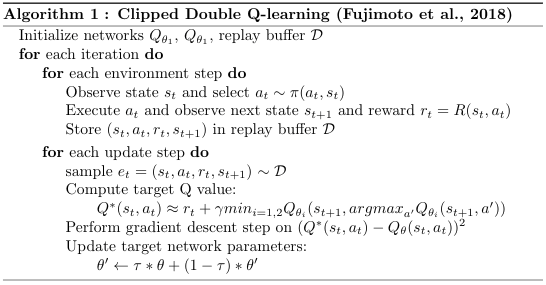
\includegraphics[width=8cm]{alg1_ClippedDDQ_Fujimoto.png}
    \end{center}
    \caption{Clipped Double Q-learning}
    \label{fig:numcomments}
\end{figure}

To evaluate results for the Clipped Double Q-learning method, we will measure its performance against Q-learning through environments from OpenAI Gym. Each algorithm will be applied to the selected environments and be run for 1 million time steps, with the average reward over 10 episodes being calculated every 5000 time steps. The max average returns for the two algorithms will be displayed in a table. Learning curves will also be shown on plots to track algorithm performance across the time step intervals.

\section{Literature Review}

The popular Q-learning algorithm is known to overestimate action values under
certain conditions. It was not previously known whether, in practice, such
overestimations are common, whether they harm performance, and whether they can
generally be prevented. Deep Reinforcement Learning with Double Q-learning
presented the background of DQN algorithm, which combines Q-learning with a deep
neural network, suffers from substantial overestimations in some games in the
Atari 2600 domain (\citet{mnih2013playing}).

In value-based reinforcement learning methods such as deep Q-learning, function
approximation errors are known to lead to overestimated value estimates and
suboptimal policies. We show that this problem persists in an actor-critic
setting and propose novel mechanisms to minimize its effects on both the actor
and critic. Clipped Double DQN algorithm takes the minimum value between a pair
of critics to restrict overestimation and delays policy updates to reduce
per-update error. We evaluate our method on the suite of OpenAI gym tasks,
outperforming the state of the art in every environment tested
(\citet{fujimoto2018addressing}).

% Import bibligraphy from ref.bib
\bibliography{ref}

\end{document}
